\documentclass[IEEEtran,letterpaper,10pt,notitlepage,draftclsnofoot,onecolumn]{article}

\usepackage{nopageno}
\usepackage{alltt}
\usepackage{float}
\usepackage{color}
\usepackage{url}
\usepackage{balance}
\usepackage{enumitem}
\usepackage{pstricks, pst-node}
\usepackage{geometry}
\geometry{textheight=9.5in, textwidth=7in}
\newcommand{\cred}[1]{{\color{red}#1}}
\newcommand{\cblue}[1]{{\color{blue}#1}}
\usepackage{hyperref}
\usepackage{textcomp}
\usepackage{listings}
\usepackage{titling}
\usepackage{graphicx}
\usepackage{url}
\usepackage{setspace}

\graphicspath{ {images/} }

\definecolor{dkgreen}{rgb}{0,0.6,0}
\definecolor{gray}{rgb}{0.5,0.5,0.5}
\definecolor{mauve}{rgb}{0.58,0,0.82}
\lstset{frame=tb,
  language=c,
  aboveskip=3mm,
  belowskip=3mm,
  showstringspaces=false,
  columns=flexible,
  basicstyle={\small\ttfamily},
  numbers=none,
  numberstyle=\tiny\color{gray},
  keywordstyle=\color{blue},
  commentstyle=\color{dkgreen},
  stringstyle=\color{mauve},
  breaklines=true,
  breakatwhitespace=true,
  tabsize=3
}

% 1. Fill in these details
\def \CapstoneTeamName{   RoboSec}
\def \CapstoneTeamNumber{   50}
\def \GroupMemberOne{     Emily Longman}
\def \GroupMemberTwo{     Zach Rogers}
\def \GroupMemberThree{     Dominic Giacoppe}
\def \CapstoneProjectName{    Security for Robotics}
\def \CapstoneSponsorCompany{ Oregon State University}
\def \CapstoneSponsorPerson{    Vedanth Narayanan}

% 2. Uncomment the appropriate line below so that the document type works
\def \DocType{    %Problem Statement
        %Requirements Document
        %Technology Review
        %Design Document
        %Midterm Progress Report
        Whitepaper
        }

\newcommand{\NameSigPair}[1]{\par
\makebox[2.75in][r]{#1} \hfil   \makebox[3.25in]{\makebox[2.25in]{\hrulefill} \hfill    \makebox[.75in]{\hrulefill}}
\par\vspace{-12pt} \textit{\tiny\noindent
\makebox[2.75in]{} \hfil    \makebox[3.25in]{\makebox[2.25in][r]{Signature} \hfill  \makebox[.75in][r]{Date}}}}
% 3. If the document is not to be signed, uncomment the RENEWcommand below
\renewcommand{\NameSigPair}[1]{#1}

%%%%%%%%%%%%%%%%%%%%%%%%%%%%%%%%%%%%%%%
\begin{document}
\begin{titlepage}
    \pagenumbering{gobble}
    \begin{singlespace}
      
\includegraphics[height=4cm]{coe_v_spot1}
        \hfill
        % 4. If you have a logo, use this includegraphics command to put it on the coversheet.
        %\includegraphics[height=4cm]{CompanyLogo}
        \par\vspace{.2in}
        \centering
        \scshape{
            \huge CS Capstone \DocType \par
            {\large\today}\par
            \vspace{.5in}
            \textbf{\Huge\CapstoneProjectName}\par
            \vfill
            {\large Prepared for}\par
            \Huge \CapstoneSponsorCompany\par
            \vspace{10pt}
            {\Large\NameSigPair{\CapstoneSponsorPerson}\par}
            {\large Prepared by }\par
            Group\CapstoneTeamNumber\par
            % 5. comment out the line below this one if you do not wish to name your team
            \CapstoneTeamName\par
            \vspace{10pt}
            {\Large
                \NameSigPair{\GroupMemberOne}\par
                \NameSigPair{\GroupMemberTwo}\par
                \NameSigPair{\GroupMemberThree}\par
            }
            \vspace{20pt}
        }
        \begin{abstract}
          In drones and other networked robotics there is a broad array of security vulnerabilities that can be leveraged in an attack.
          We will evaluate ROS to find as many of these security holes as we can and document them.
          The different vulnerabilities found will be categorized into malware, sensor hacks, network and control channel attacks, and physical breaches.
          For some of these exploits we may be able to implement solutions, which will also be documented.
          These findings and any solutions will be added to an ongoing academic effort to make robotics more secure.
        \end{abstract}
    \end{singlespace}
\end{titlepage}
\newpage
\pagenumbering{arabic}
\tableofcontents
% 7. uncomment this (if applicable). Consider adding a page break.
%\listoffigures
%\listoftables
\clearpage

\section{Introduction}
Robotics is still a relatively up and coming field and as most efforts in robotics are in pursuit of furthering capabilities, security has been left largely untouched.
Because of this many functioning, deployed robots have limited to no security in their internal systems, making them very vulnerable to attacks.
While the community developing robotics is still largely academic and there is little worry of being attacked, the security vulnerabilities still exist.
Soon robotics will become ubiquitous in society and hackers will exploit these vulnerabilities for personal gain.
There have already been reports of smart appliances being used for botnets, it's only a matter of time before drones and other robotics are similarly abused. \cite{ddos}
This project aims to eliminate some of this abuse before it begins.

\section{Problem Statement}
%ROS is known by many users to be insecure, but until now nobody had made any serious effort to document in which ways it is insecure.
%Our group undertook an exploratory effort to document ways we found it to be insecure as a starting point for what could be a more thorough documentation of the variety of ways it is insecure, for future research or development.
%This paper summarizes our findings.

Since robotics are continually in development and there is such a wide variety of devices, focus needed to be on a small subset of robotics to have any hope of making progress within a year. 
Because of this the Robotic Operating System (ROS) was chosen for this project.
These operating systems can be attacked at the driver level with malware, they can have the configuration files modified, and they can have data intercepted or spoofed in their internal communication subsystems.
We could also investigate the ability to spoof sensor data, such as the camera, IR guidance, accelerometer, or gyroscopic systems. 
Outside of the OS level there is a huge amount of room for exploitation in the communication and control channels used by networked devices. 
It's very important that we acknowledge all of these risks, since exploitation of them could be a big setback for global trust of robotics.

Essentially the problem is twofold; first a specific feature of a specific device needs to be isolated, and then that feature needs to be broken, and all work documented.
This could be a crucial improvement for the use of robotics running ROS in a wide variety of sectors.
The military uses and plans to use them widely, and for them more than anyone they need to be as secure as possible.
Amazon and other commercial shipping companies have a vast use of robotics, and we've all heard about their plans for delivery drones, which are a huge security risk.
If consumers think these will be abused they won't trust this upcoming technology and it will be slowly or never adopted, which will make companies hesitant to invest in their development.
Consequentially, the world as a whole will be slower to advance robotic technology.
Hopefully our work in securing robotics can help to better develop consumer trust in this emerging technology.

\section{Literature Review}
This project would have been much more difficult without a variety of documentation and previous research into the security of ROS and robotics in general.
One paper that was widely used in the creation of our project basis was \"A Preliminary Cyber-Physical Security Assessment of the Robotic Operating System (ROS)\". \cite{mainROS}
This article was written by a group of researchers who created a honeypot robotic system and brought it to DefCon 20 to let hackers there exploit it as they could.
This lead the researches to be able to recored a range of attack vectors from a wider variety of minds.
They also used a number of their own methods to study what was being done, such as examining the packets being sent and received through wireshark, visualizing the effects with hardware, and using Backtrack Linux.
Their work provided starting points for many different ways to attack the system, and for cataloging the effectiveness of each different type, relative to the others.
The inspiration from this paper laid a groundwork for the threat models that would be created here, and for the exploratory structure that was followed.

One particularly useful paper was written by Bernhard Dieber et al, which discussed security on the application level of ROS.
It provides great insights for the problems with authentication and data integrity that are present in ROS. \cite{App}
This helped to provide guidance for that portion of our model, and was foundational in the understanding of how the application level interacts with the rest of the system, from a security standpoint. 
A similar paper entitled \"ROS: an open-source Robotic Operating System\" was vastly useful in the planning of this project, as it gave a detailed overview of the system from a research standpoint.
while the official site and documentation of ROS was absolutely invaluable, this paper provided us with a third party assessment of the system and how all portions work together.
Without a thorough understanding of this research would be much more difficult. \cite{Open}
 
The last of the papers that were used extensively in the overall planning and implementation of this project was one discussing the SROS project.
This project is very closely aligned with ours in that they are working to bring better security to ROS in its most vulnerable sectors.
The areas in which this project most wanted to provide security were some of the first that our project investigated. 
Specifically it provided insight into the access control policies needed in ROS, the insecurity of the communication channels, and they way in which processes are handled. \cite{Sros}

To find inspiration for specific exploits that would be created, a lot of other research papers, journal articles, and security presentations were examined.
These are referenced and discussed within each of packages to which they contributed.

\section{Threat Model}
A key element to our project is being able to accurately find vulnerabilities or identify areas where they are likely to be.
One of the best ways to do this in an organized way that can be later referenced is with threat modeling.
Adam Shostack has a well defined method for doing this, which was followed to develop the model for this project. \cite{TMDS}

An important thing to note is that ROS is middleware, which means it sits between the base Linux OS, and the application level.Typically there is little focus on security because middleware like this needs to be lightweight. 
Without any specific security measures taken, there is room for all manner of attacks. To try to tackle them, the vulnerabilities were broken into the three categories of the CIA Triad \cite{CIA}:
\begin{itemize}
  \item Those affecting the confidentiality of data
  \item Those affecting the integrity of data
  \item Those affecting the availability of data
\end{itemize}

A threat model was created to visualize these three categories. It serves as a roadmap for the research and can be looked back on at any time.
The model below in Figure 1 is organized as a tree, with the three main branches being the three components of the CIA triad (Confidentiality, Integrity, and Availability).
This way one can look at our threat model, decide if their concern is one of confidentiality, integrity, or availability, then examine the vulnerabilities in that category.

\begin{figure}[H]
    \centering
    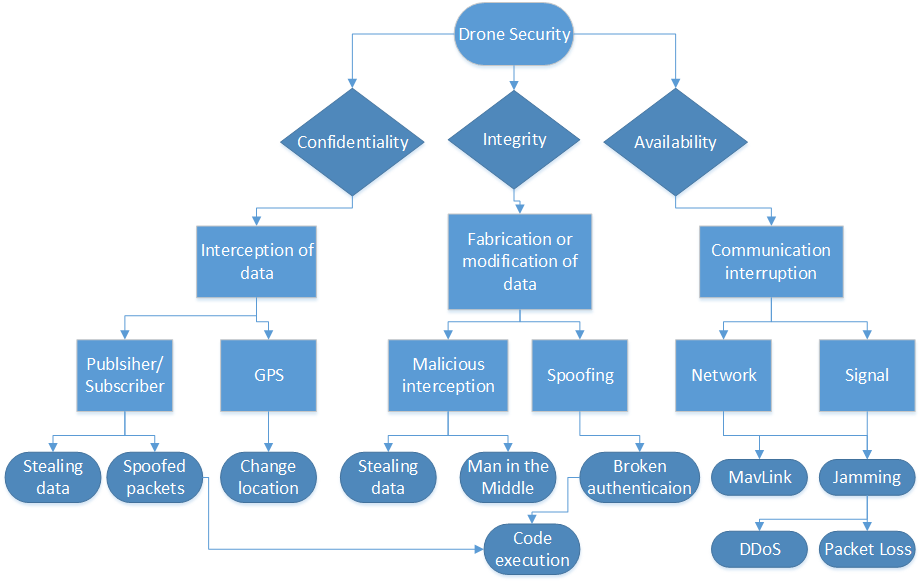
\includegraphics[width=\textwidth]{model}
    \caption{A view of the attacks that are viable against the ROS system}
\end{figure}

Not every area from the threat model was successful, some were not possible to breach, but it is important to acknowledge their importance.
This new version of the threat model was created to showcase the success level of each area using color coding.
Those areas that are red have a lot more potential for vulnerabilities, yellow has been covered by our research but is still likely to have more, and green was heavily covered and only an expert in that area would be likely to identify more.
This also includes our specific packages as leaves, rather than the general concepts they covered.

%\begin{figure}[H]
%    \centering
%    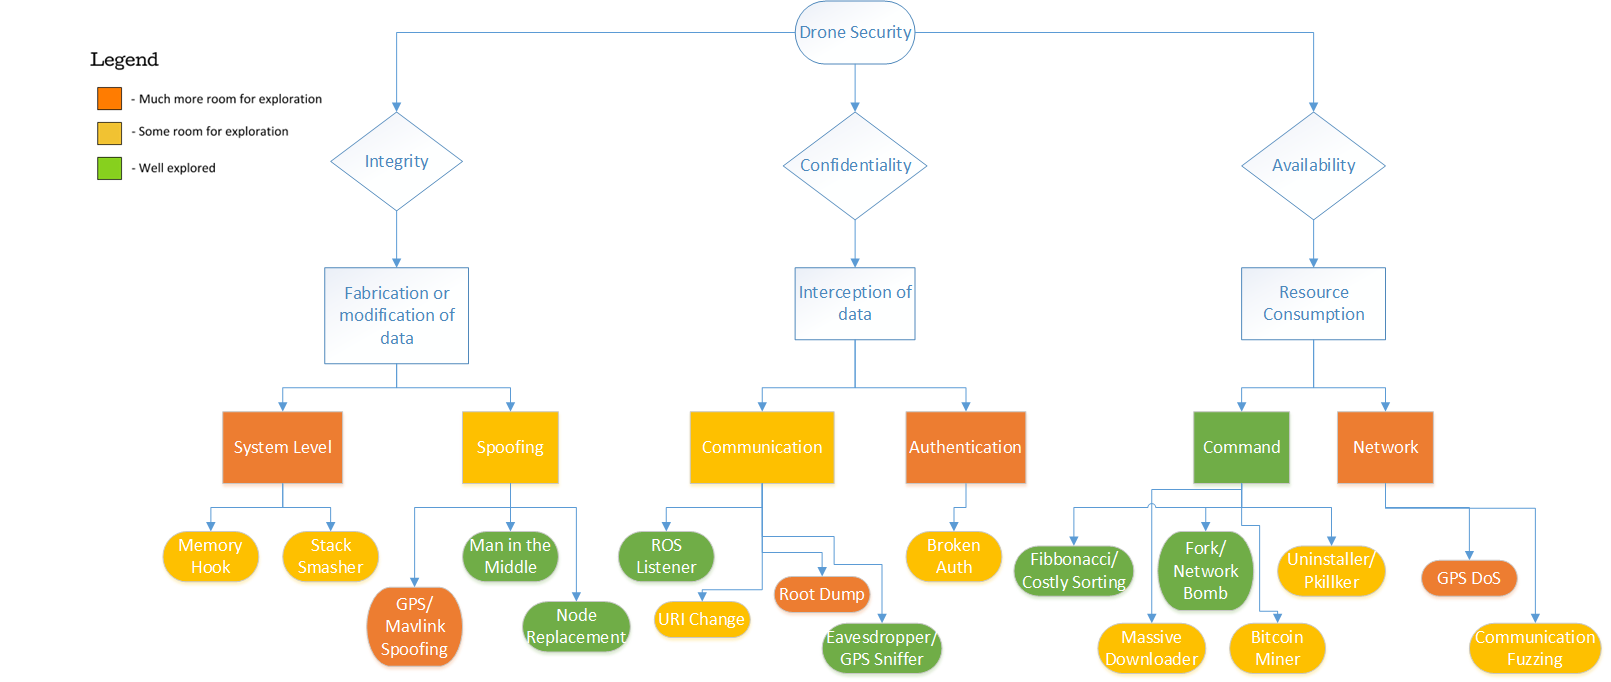
\includegraphics[width=\textwidth]{color_model}
%    \caption{map of the areas which were most or least covered in this research}
%\end{figure}

\section{Packages and Solutions}
As mentioned above, the exploits written were meant to cover a lot of ground topic wise.
Some are based on the same vulnerability, while others are more distinct.
Specific packages have been chosen below to represent each of the notable categories of attack.
These range from resource consumption, to network sniffing and spoofing, and to OS level exploitation.

\subsection{Eavesdropper}
Called Malpac in the repo, this is a very simple package. It has 2 nodes, one that publishes a string every couple seconds, and 
a subscriber that takes that message and prints it to stdout. There is also a third “malicious” node which also subscribes to 
the publisher and prints the same message with a slight modification to stdout as well. While not that malicious in this case, 
the general principle can be used to receive and change any published data, including sending said data to other computers 
using the ROS subscriber/publisher system and compromise the original data’s integrity.
For example, if you had a drone doing aerial reconnaissance of an area and transmitting the images back to a base, this kind of 
system would be able to intercept those images.

\subsection{Forkbomb}
This package is a forkbomb.
As stated previously there is no process monitoring or control native to ROS, so this is a very simple forkbomb. All it does is 
do a little math to slow things down a bit, then call itself 8 times and exit.
Eventually there are enough processes to clog the CPU and cause a kernel panic, bringing down the robot.
In theory, as long as you don’t have some sort of process management, this would kill any robot with enough time, which has 
obvious use cases.

\subsection{Network Bomb}
This exploit temporarily disables the operating system's wireless networking capabilities.
For a robot dependent on wireless communication for control or navigation, this has some rather obvious consequences.
Depending on how the robot handles the lack of networking it could do anything from fall out of the sky to automatically
returning home. It could also permanently disable the wireless networking with a small tweak, which would make the only 
fix to physically capture and wire back into the robot to fix the networking. 
Either way, if one's robot is dependent on wireless networking, it will be downed for a bit.

\subsection{Fibonacci}
This one is actually our Client, Vee's package. It does a naive recursive implementation of the calculation of Fibonacci
numbers, and tries to calculate the 100000th number. It either takes a long time, or stack overflows and crashes, neither 
of which being terribly great results and both using a fair amount of system resources. As such it has the potential to 
bring down the system, depending on how exactly python handles the recursion involved, or at least be a waste of resources 
for a bit.

\subsection{Local Folder}
This package just creates and then deletes a local folder. In theory it can delete any user level folder, which may include
program files or ROS nodes or maybe just something important locally. If it has super user permissions then it could go so
far as delete system directories or the like, but that is not guaranteed. Either way it can probably delete something that
the user would rather it not.

\subsection{Node Replacement}
Consisting of 2 parts, this includes one package which launches a publisher that publishes a string every couple seconds and a 
subscriber that takes that string and prints it to stdout.
The other one runs a package that kills the subscriber from the 1st package, and replaces it with its own subscriber with the 
same name that prints a modified message to stdout.
At the time we thought the node would be indistinguishable from the previous node besides the different message, but it turns 
out that ROS silently assigns each publisher and subscriber its own unique ID and is in fact quite noticeable.
It might be hard to notice by an inattentive user, assuming they do not notice the slight hiccup where the old subscriber dies 
and is replaced, so it still has potential to be a threat or phone home.

\subsection{Costly Sorting}
This is a package that performs bogo-bogo sort. \cite{bogo}
Bogo-bogo sort is an extremely inefficient sorting algorithm that performs a random shuffle to sort a list, recursively.
While it is not particularly system intensive, the sort for a list with a mere 10 elements can take on the order of days.
The goal of this package was not to be directly malicious but more of a lurking threat; it shows that ROS also does not check 
for any particularly long running processes, which allows for a variety of actual threats. It also wastes some CPU time.
The best example is an attack that lies dormant until signaled to do maximum damage, or one that waits for a specific process 
to kill it.

\subsection{URI Change}
This is a package that changes the ROSMASTER URI to an arbitrary one, and starts a new ROS master to match.
The URI is basically where packages check for the ROS master node, which is the master in the ROS master/slave system.
ROS master manages nodes, and the publisher/subscriber system between nodes as its 2 main duties.
As such, changing the URI and starting a new ROS master node means that all new nodes will talk to the new ROS master as 
opposed to the old, which could allow for some interesting node management or fiddling with the publisher/subscriber system.
The ROSMASTER URI can also be set to a remote machine if it setup correctly as well, which means you could have a compromised 
robot respond to a remote ROS master node as well, allowing an attacker to control the robot remotely.

\subsection{Pkiller}
This simply pkills (process kill, for those unfamiliar) all processes with ROS in the name.
This will at least kill ROS master, and maybe some other related ROS processes, but killing ROS master also kills all the nodes currently being managed by ROS master, so it will also kill all ROS processes on the system.
This has the obvious effect of bringing the robot to a halt, and has the potential of doing major damage.
Just image if a drone carrying an explosive payload fell out of the sky because its control system suddenly stopped.

\subsection{Massive Download}
This package uses wget to attempt to download all of Wikipedia.
It probably will not succeed, unless the robot has enough disk space to hold all of Wikipedia, but it will fill the disk up to 
the limit. This can cause a number of issues depending on what else needs disk space, but it is sure to cause some sort of 
issue. If nothing else it will prevent any more ROS processes from being launched, as ROS master does some record keeping for 
each process and will need a little disk space for that purpose.

\subsection{Root Dump}
This package dumps your filesystem to a remote machine, currently a dummy address. If you had something confidential on the
robot, it is now in the hands of some other party, assuming your network connection did not die mid-transfer or something.
If your drone had those top secret recon images, or maybe the drone's code itself was supposed to be a secret, they could
potentially be in the hands of some unknown party.

\subsection{Uninstaller}
This one, assuming your ROSMASTER was run with root privileges and is on a Linux distribution that uses apt-get as its package
manager, uninstalls ROS from the robot. The robot's operations will be unaffected until next boot as the ROS binaries will be 
loaded into system memory, but on reboot or if ROS is killed and restarted in some other way, ROS will no longer be there.
Especially bad if the ROS install was customized, as one would have to redo all those configurations all over again...

\subsection{Start WW3}
This pings (what the team knows to be, but can not directly confirm) a North Korean IP address. 
While it has no direct effect on the system, alerting North Korea to your presence is not exactly a great idea in the current political environment, and has a good chance of getting one on a watchlist. 

\subsection{Bitcoin Miner}
This package attempts to install a bitcoin mining service on the robot.
It does currently need superuser permissions for this, as it does need to use apt-get, which means that ROSCORE 
needed to be run as a superuser so that this child process would have those permissions as well.
If the install succeeds however, then you have a bitcoin miner using CPU time for someone else’s monetary gain, and with a 
little more work could be further configured to have the miner run at boot as a system process, but for the purposes of the 
package it was good enough as is.

\subsection{ROSless Listener}
Here was an attempt to abuse how ROS subscribers and publishers really worked outside of ROS.
All subscribers and publishers actually communicate through a shared TCP/UDP socket controlled by ROS master, and the general 
idea was to make a non-ROS socket to communicate with the ROS socket, subscribe to a known publisher on the ROS machine, and 
print whatever they published as plain text to stdout.
In short, something like the first malpac, but going around ROS to do so. Unfortunately ROS uses TCP/UDP with a special header encoding that makes this difficult, as to communicate any publisher or subscriber you need their unique ID, which is assigned to them by ROS master at their launch. And to get said ID, you need to do some handshaking with ROS master, which turned out to be a bit beyond our technological capacity and time constraints.
We believe it is still possible to achieve this, but to do so would require a better working knowledge of sockets and more 
investigation into the handshake protocol used by ROS master.
While the documentation is available online, specifically on the technical overview page of the official ROS site \cite{ROS}, it was just a little too much for the team with the time we had. Malpac ROS is similar to this, but differs in that Malpac ROS 
still uses ROS to achieve this goal, while this package aimed to bypass ROS entirely.

\subsection{Linux Kernel Exploitation}
This package contains two scripts, a memory hook and a stack smasher.
The first, the memory hook, is actually a Linux kernel exploit, and doesn't use ROS itself, but ROS commonly sits atop Ubuntu or Ubuntu-based linux systems.
This package does a simple memory hook into the syscall table, which allows the script to make changes to whichever syscalls it wants once it finds the syscall table memory address.
This is done by changing the pointer to the function of an existing syscall and replacing it with a pointer to a malicious function.
This is the kind of script that would likely be secondary to one of the network attacks. One of those might be used to get into the system, and could then install LKMs like this one. Since it operates at the kernel level in Linux, ROS would have no way of ever knowing something was amiss, which renders this a very insidious threat.

The second script, the stack smasher, provides a basic proof of concept (PoC) for stack smashing.
This is a form of buffer overflow attack which has been used reliably for a very long time to gain unauthorized access to a system.
It works by leveraging the overflow to push its way into privileged space and then execute some form of malicious code once it has entered that area of the stack.
This specific script is a small scale buffer so better demonstrate the idea.
To use a simple approach like this, one needs access to the environment variables of the system so it's not perfect.

\subsection{GPS Exploitation}
The exploits in the category work with the GPS or Mavlink protocol.
Specifically the GPS package uses both spoofing and man in the middle to trick a drone into thinking it is the home base, and can misguide it.
This is done by sniffing for drone network information, and then leveraging that to send spoofed landing data via UDP.
The Mavlink script follows the same idea, but it was never able to reach a point of development beyond simply sniffing for the information and positioning itself as a node in the middle.
With better documentation and a system with which to reliably test it the Mavlink script could grow to the point of the GPS one.

\subsection{ROS Broken Authentication PoC}
\begin{figure}[H]
  \centering
    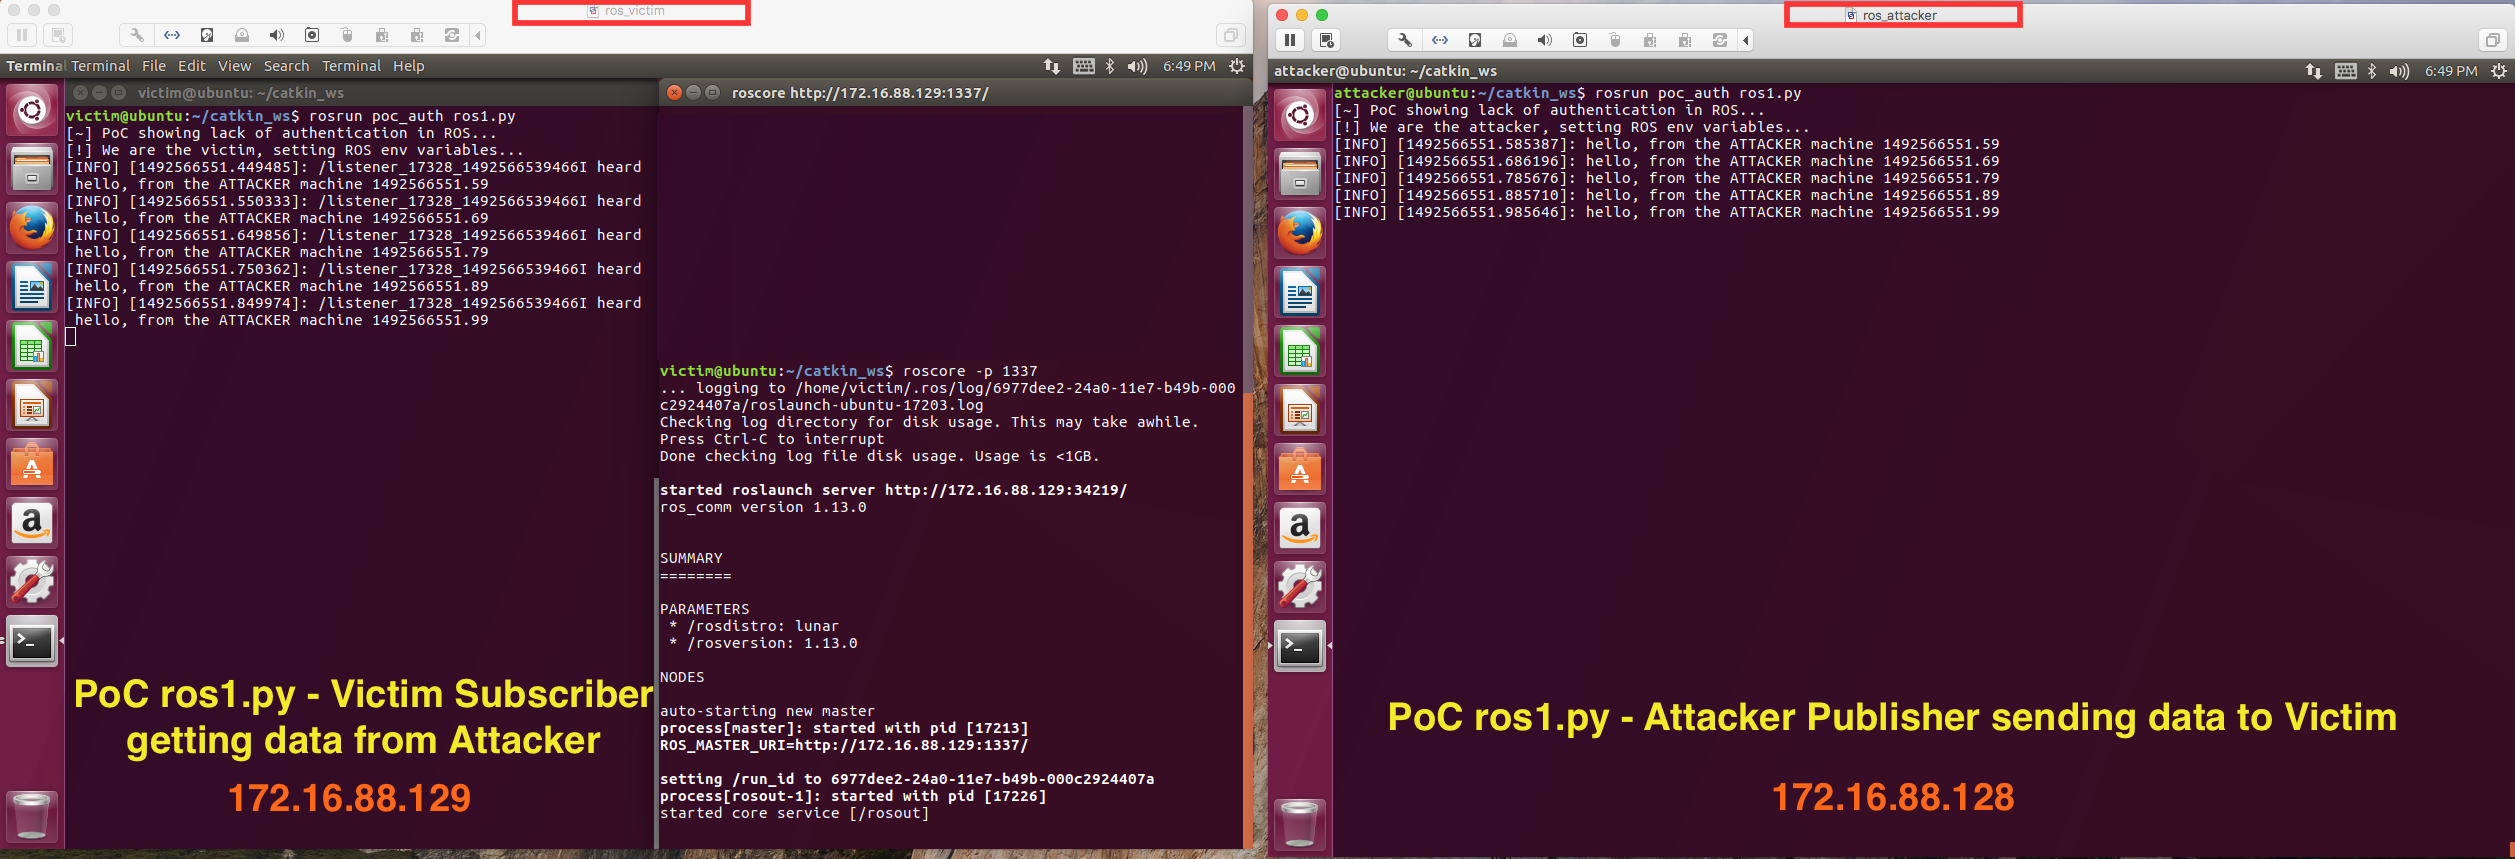
\includegraphics[width=\textwidth]{poc1}
    \caption{PoC ROS Broken Authentication}
\end{figure}

Two PoC packages were created that show ROS has zero authentication measures, by leveraging the publisher subscriber model.
These simple yet effective PoCs are the basis for remote ROS exploitation. If you know the IP address of a remote ROS machine, you can leverage it as you wish, without the need
to authenticate with the machine in any way. This should not be taken lightly, as this opens up ROS to any device that has a network connection. The PoC proving this to be true
connects to a remote \"victim\" machine, sending data to a ROS subscriber process. This complete PoC package extends upon Malpac 8 and 15.

\subsection{ROS Process Communication}
\begin{figure}[H]
  \centering
    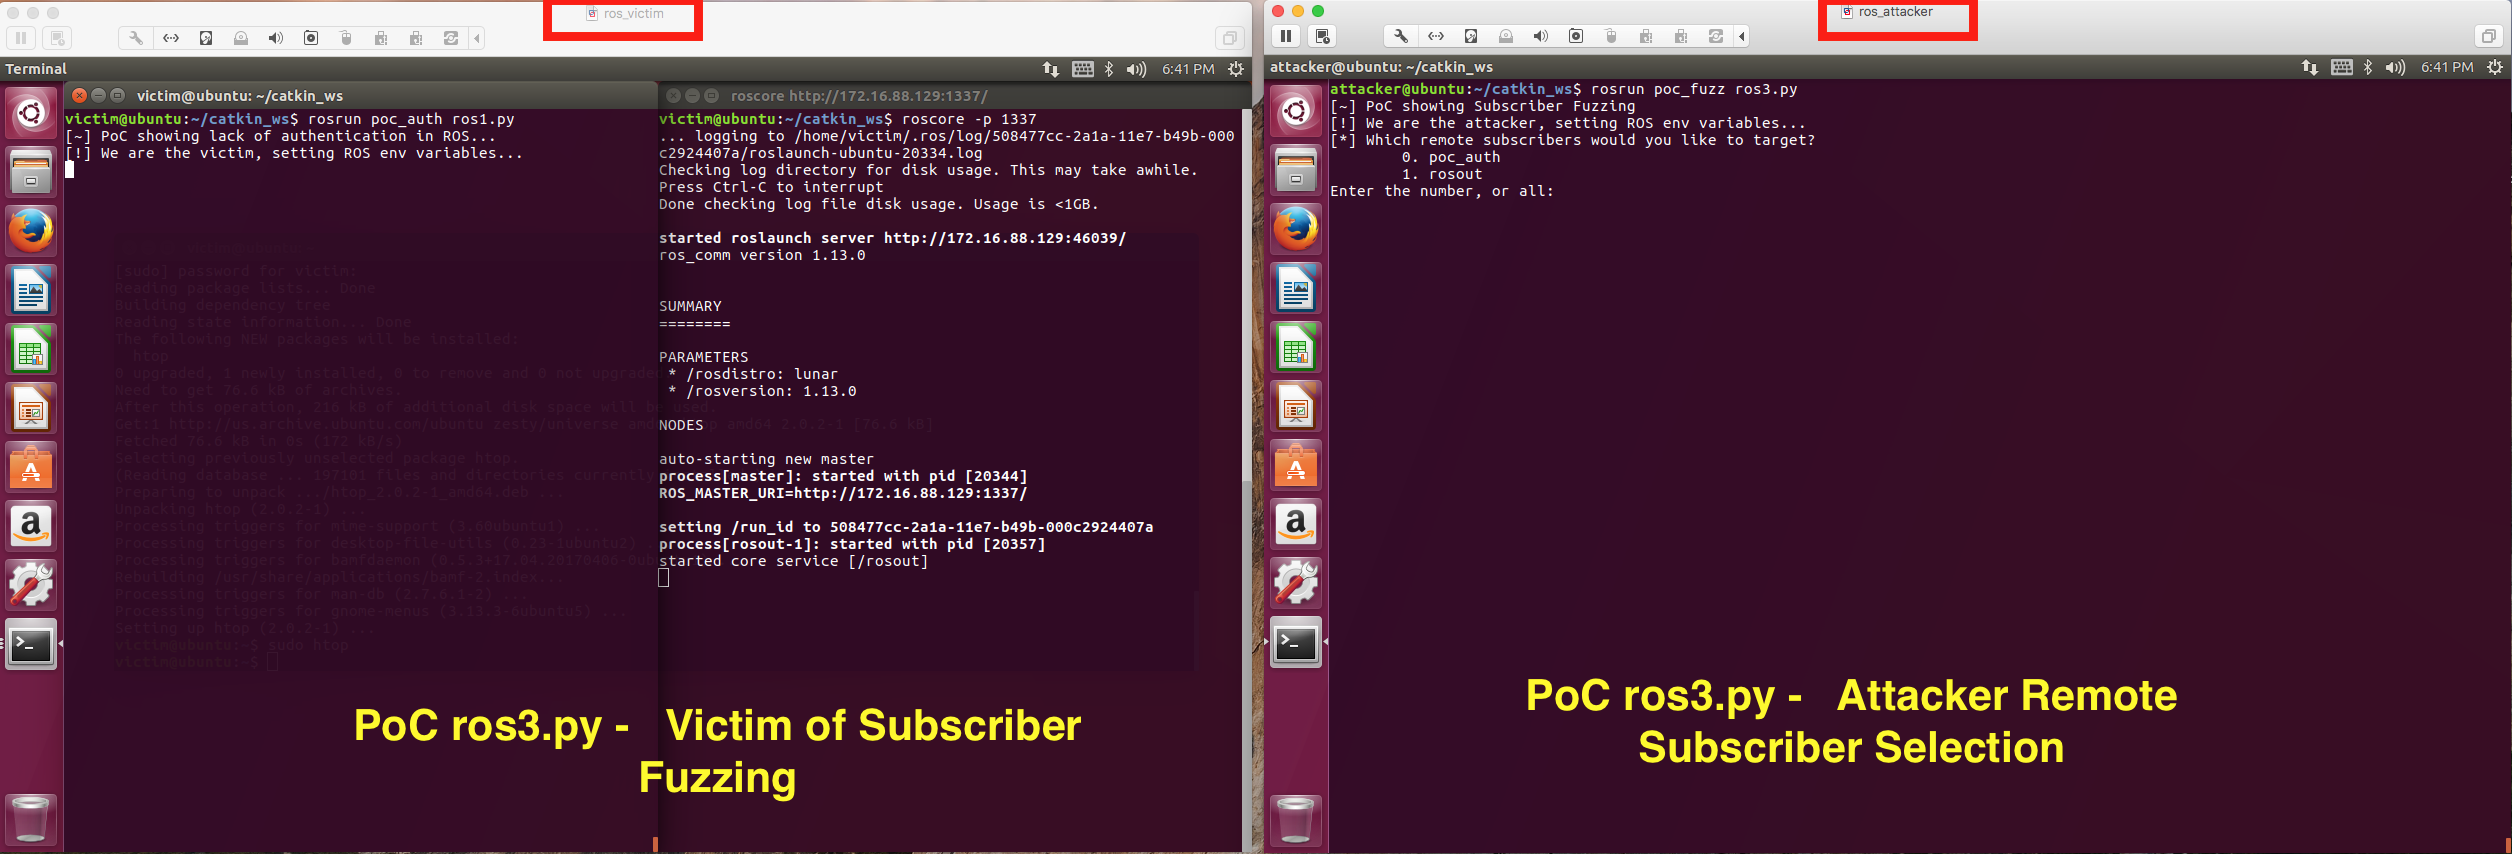
\includegraphics[width=\textwidth]{poc2}
    \caption{PoC ROS Fuzzer Selection}
\end{figure}

Two additional packages were created, exploring exploitation of the process communication model that ROS uses. These PoC packages act as ROS security tools, one of which is a subscriber
fuzzing tool, and the other a publisher data capture tool. The subscriber fuzzer allows an attacker to target remote ROS processes by flooding them with large amounts of malformed data.
This can be used to expose issues with ROS processes on a real world device, like a drone. The remote publisher data capture tool uses a ROS tool called rosbag to create a saved instance
of a given ROS process. This PoC uses that data to preform what's known as a \"ROS Bag Replay Attack\", which can cause devices running ROS to carry out a given operation at the will of the attacker.
For example, an attacker could capture what happens with a drone flight control process turns on the motors to begin flight. The attacker could then \"replay\" that action remotely, causing the drone
to fly. It is also possible to modify this captured data before replaying it via ROS, so an attacker could replay a malicious payload quite easily using this method.

\begin{figure}[H]
  \centering
    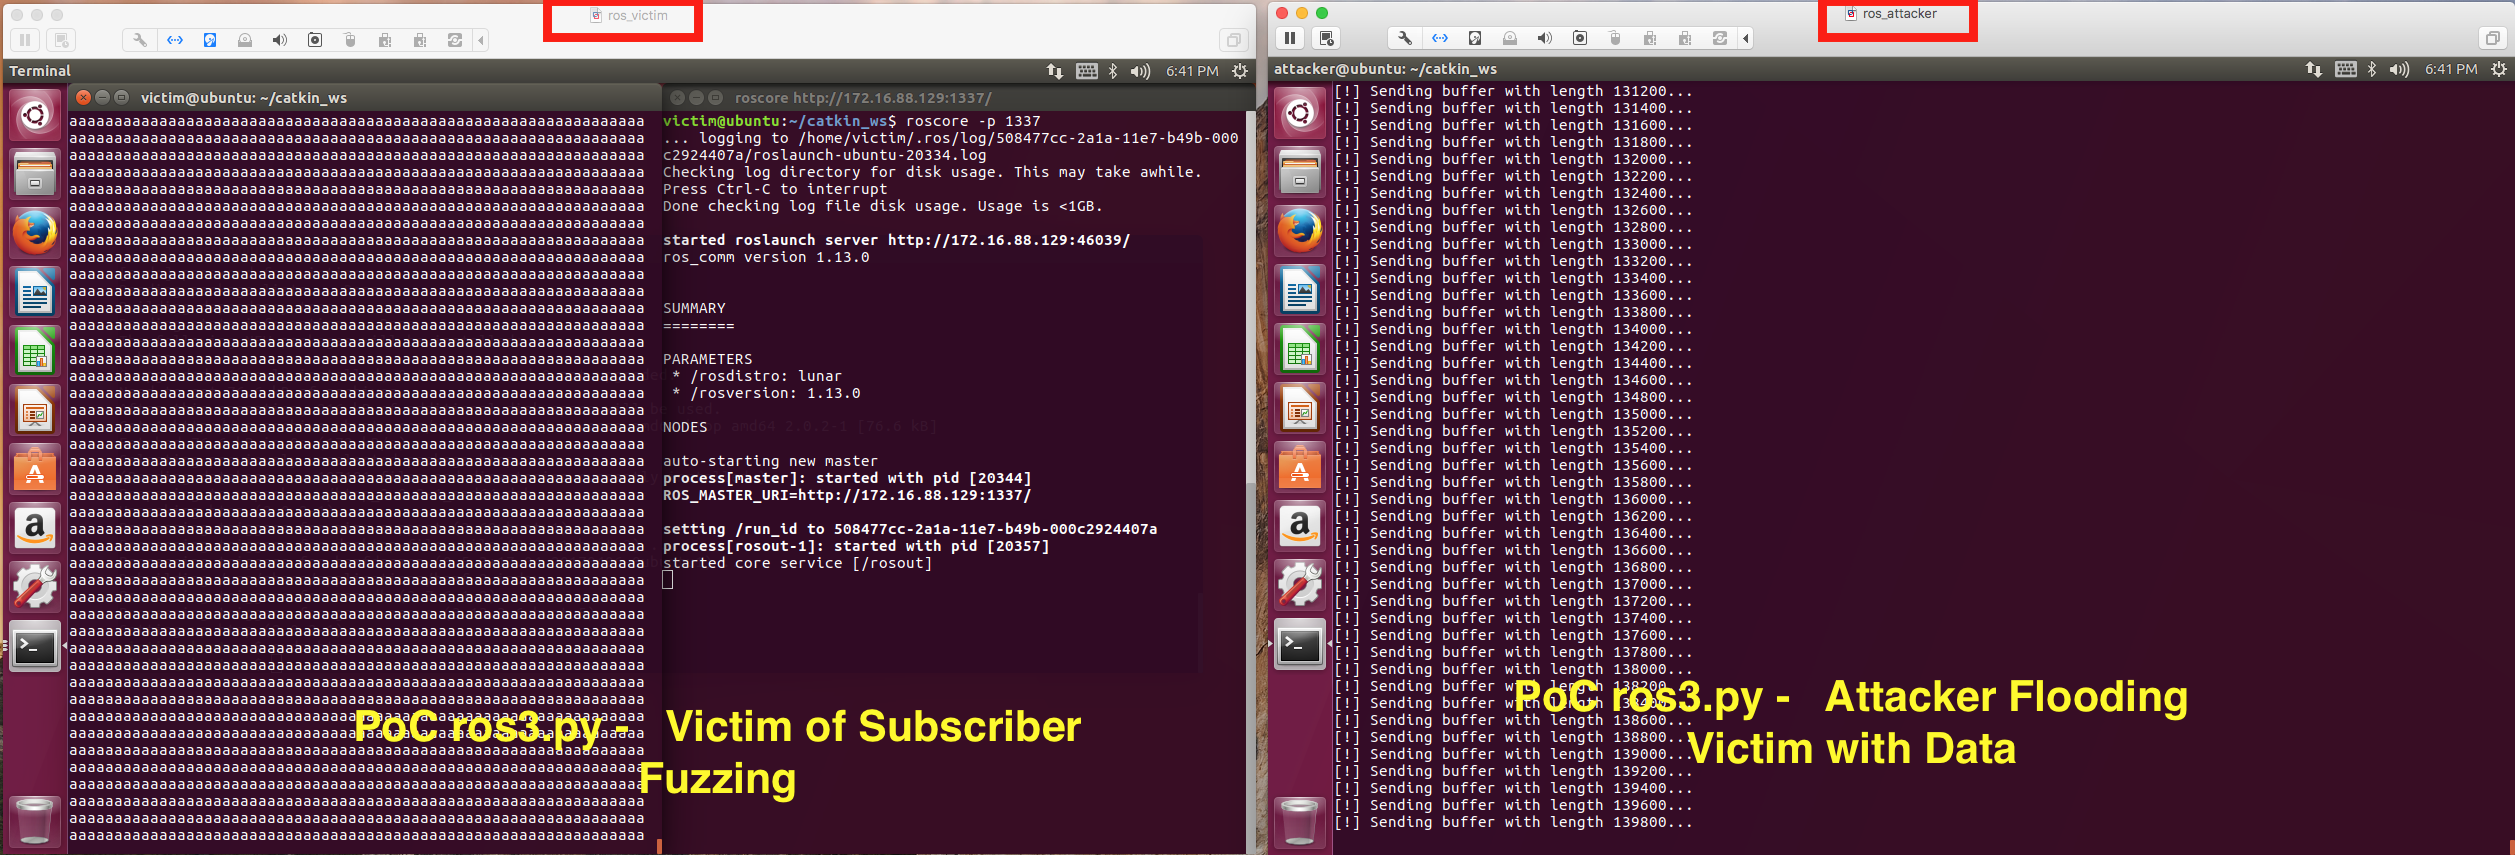
\includegraphics[width=\textwidth]{poc3}
    \caption{PoC ROS Fuzzer Execution}
\end{figure}

\section{Testing Methods}
Failure Mode Effects Analysis (FMEA) is a procedure used in a variety of fields which creates an empirical system for testing and logging any failures, which can be applied to all of our attacks. \cite{FMEA}
Somewhat akin to risk analysis, FMEA involves defining severity, occurrence, and detection rating scales, usually from 1 to 10.
After these scales have been defined one can use them to calculate a risk priority number (RPN) and a criticality number with which the found failures can be ranked in order of importance.
You can see this represented in figure 5 below.

\begin{figure}[H]
    \centering
    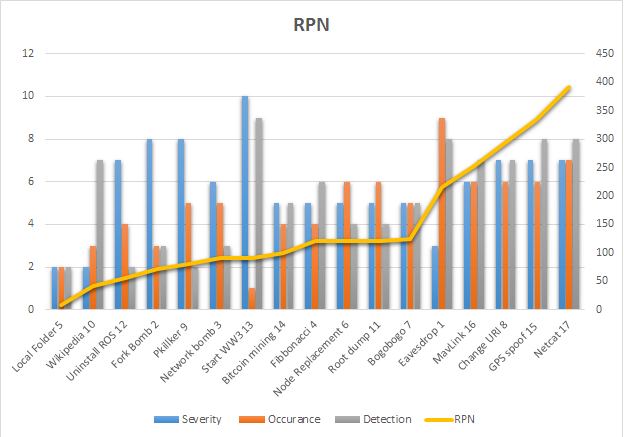
\includegraphics[width=\textwidth]{RPN}
    \caption{The increasing criticality ratings of packages, based on the three combined numbers}
\end{figure}

\section{Limitations}
The main limitation our project faced was not being able to do testing on actual robotic hardware.
If this project were continued, the next steps would be to setup a ROS enabled drone and see how our exploit packages effect the drone's functionality.
Testing on real world hardware will drive home the real-world implications of using an insecure middleware on robotic devices with open communication channels.
Our research is not just limited to drones; any device running ROS can be used to further test our methods.
While our testing was done on ROS enabled machines, those machines were not real-world robotic devices, thus the real-world impact of our packages could not be evaluated.

\section{Findings}
Just as suspected, ROS has wide range of vulnerabilities that this project exploits with a success rate of nearly 100\%.
Most of these exploits involved either entering the system via the publisher/subscriber system that ROS uses to communicate, or demonstrated what malicious actions could take place on the system once inside.
Those that interrupted the availability of the system were most prevalent, since it's somewhat trivial to break subsystems once inside.
The next most common type of exploit was those that tamper with the integrity of data, usually in network communication.
The least common were those that broke the confidentiality of data, often through authentication or sniffing.

We also found that our project evolved as we went along.
We had initially intended to do more hardware based attacks, but they proved to be too cumbersome and difficult to generalize.
There are also a board range of physical attacks ranging anywhere from an EMP type gun to an eagle taking down an airborne drone.

\section{Analysis}

\section{Future Research}

\section{Conclusion}
ROS is vulnerable in at least the ways detailed above, and as such is insecure.
There are also vulnerabilities whose existence we are confident of, but were unable to write code to exploit in the given time.
In particular, due to our inability to repair our test drone in time, we were unable to attempt any exploits involving hardware.
Most of the vulnerabilities come from basic design choices and philosophy in ROS itself, and to attempt to fix said vulnerabilities would take fundamental changes and re-designs in ROS.
There are indeed already undertakings to do just that, specifically SROS and ROS2, but overall it is probably better to design drone security around the fact that ROS is insecure, if one chooses to use ROS, than attempt to fix ROS itself.
Many of our vulnerability exploits come from having access to ROS itself or by abusing lax communications security to get into ROS, so just ensuring that the ROS is only accessible by trusted users is enough to prevent most exploits that we have found, although that in itself is a rather big task.

\bibliographystyle{IEEEtran}
\bibliography{research.bib}

\end{document}
